\documentclass[11pt]{article}
\usepackage{amssymb}
\usepackage{amsthm}
\usepackage{enumitem}
\usepackage{physics,amsmath}
\usepackage{bm}
\usepackage{adjustbox}
\usepackage{mathrsfs}
\usepackage{graphicx}
\usepackage{siunitx}
\usepackage[mathscr]{euscript}

\title{\textbf{Solved selected problems of Classical Mechanics - Gregory}}
\author{Franco Zacco}
\date{}

\addtolength{\topmargin}{-3cm}
\addtolength{\textheight}{3cm}

\newcommand{\hatr}{\bm{\hat{r}}}
\newcommand{\hatx}{\bm{\hat{x}}}
\newcommand{\haty}{\bm{\hat{y}}}
\newcommand{\hatz}{\bm{\hat{z}}}
\newcommand{\hatth}{\bm{\hat{\theta}}}
\newcommand{\hatphi}{\bm{\hat{\phi}}}
\newcommand{\hatrho}{\bm{\hat{\rho}}}
\theoremstyle{definition}
\newtheorem*{solution*}{Solution}
\renewcommand*{\proofname}{Solution}

\begin{document}
\maketitle
\thispagestyle{empty}

\section*{Chapter 9 - The energy principle and energy conservation}

	\begin{proof}{\textbf{9.1}}
        First, we want to calculate the potential energy that comes from the 
        uniform gravity which is given by
        \begin{align*}
            V = mgZ_Q + MgZ_P
        \end{align*}
        Where $Z_Q$ and $Z_P$ are the vertical displacement of $P$ and $Q$
        against $O$. Then we have that
        \begin{align*}
            Z_P = a \cos(\theta) \quad\quad Z_Q = a \cos(\frac{\pi}{2} - \theta)
        \end{align*}
        Then
        \begin{align*}
            V = ga(m\cos(\frac{\pi}{2} - \theta) + M\cos(\theta))
        \end{align*}
        We must now show that the constraint forces do no work. The rate of
        working of the constraint force $\bm{R}$ that the cylinder exerts on
        each of the particles is $\bm{R} \cdot \bm{v^Q} + \bm{R} \cdot \bm{v^P}$
        where $\bm{R}$ is perpendicular to both $\bm{v^Q}$ and $\bm{v^P}$
        therefore the rate of working of $\bm{R}$ is zero.
        Also, the internal constraint forces that enforce the rigidity of the
        light inextensible string does not work in total. Hence, the constraint
        forces do no work in total.

        Therefore energy conservation applies in the form
        $$T + ga(m\cos(\frac{\pi}{2} - \theta) + M\cos(\theta)) = E$$
        The equilibrium position happens when $V' = 0$ then it should happen
        that
        $$m\sin(\frac{\pi}{2} - \theta) - M\sin(\theta) = 0$$
        and this is true when $\theta = \tan^{-1}(m/M)$

        It follows that the equilibrium position will be stable if $V$ has a
        minimum there, to check this we calculate $V''$ and we replace the
        value of $\theta$ we got there, then 
        \begin{align*}
            V'' &= -ga(m\sin(\theta) + M\cos(\theta))\\
                &= -ga(m\sin(\arctan(\frac{m}{M})) + M\cos(\arctan(\frac{m}{M})))\\
                &= -ga\sqrt{m^2 + M^2}
        \end{align*}
        Since $V'' < 0$ then $V$ does not have a minimum there. Therefore
        the equilibrium point is not stable.
    \end{proof}
	\begin{proof}{\textbf{9.2}}
        Just to clarify, the system looks like this
        \begin{center}
            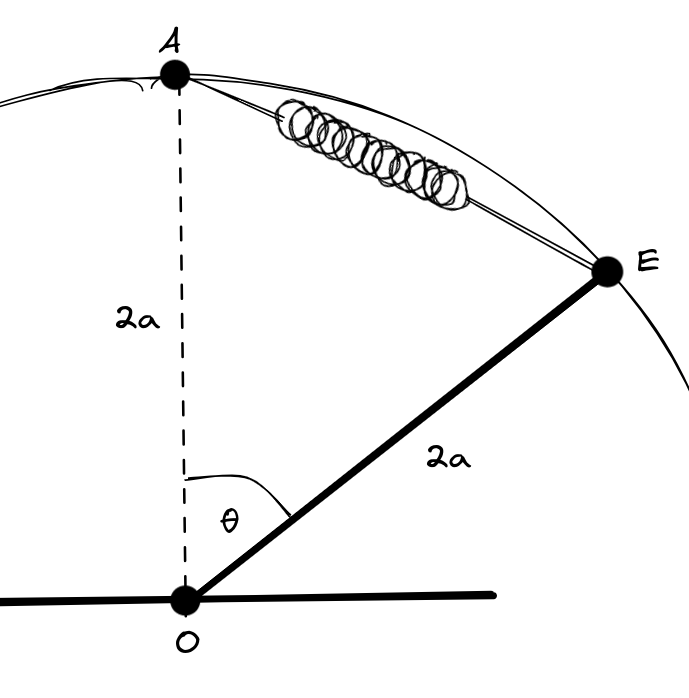
\includegraphics[scale=0.4]{ch9-2.png}
        \end{center}
        
        We want to calculate the potential energy of the system.
        There are two contributions to the potential energy, the uniform
        gravity exerted on the rod and the spring elasticity. Then we have that
        \begin{align*}
            V = mgZ + \frac{k}{2}X^2
        \end{align*}
        Where $Z$ is the vertical displacement of the rod's center of mass,
        $X$ is the net displacement of the spring over or under the natural
        length $a$, and $k = \frac{mg}{2a}$ is the spring constant. 
        From the image, we see that $AE$ is a chord of the circular trajectory
        into which the rod is moving so we have that
        $$AE = 4a\sin(\frac{\theta}{2})$$
        Then $X =4a\sin(\frac{\theta}{2}) - a = a(4\sin(\frac{\theta}{2}) - 1)$.
        On the other hand $Z = a \cos \theta$ then we have that
        \begin{align*}
            V &= mga\cos\theta + \frac{1}{4}mga
            \left(16\sin^2\left(\frac{\theta}{2}\right)
                -8\sin(\frac{\theta}{2}) + 1\right)\\
                &=\frac{1}{4}mga\left(4\cos\theta + 16\sin^2\left(\frac{\theta}{2}\right)
                -8\sin(\frac{\theta}{2}) + 1\right)\\
                &=\frac{1}{4}mga\left(4 - 8\sin^2\left(\frac{\theta}{2}\right)
                    + 16\sin^2\left(\frac{\theta}{2}\right)
                    -8\sin(\frac{\theta}{2}) + 1\right)\\
                &=\frac{1}{4}mga\left(8\sin^2\left(\frac{\theta}{2}\right)
                    -8\sin(\frac{\theta}{2}) + 5\right)\\
                \end{align*}
        The equilibrium point will happen when $V'=0$ then
        \begin{align*}
            4\cos\left(\frac{\theta}{2}\right)\left(2\sin(\frac{\theta}{2}) - 1\right) = 0
        \end{align*}
        This means that the equilibrium points happen at $\theta = \pi$ and
        $\theta = \pi/3$.
        To find out if they are stable we need to check that $V$ has a minimum
        at these points so we compute $V''$ and we check the signs of $V''$ then
        \begin{align*}
            V'' = 2(2 \cos^2(\theta/2) + \sin(\theta/2) - 2 \sin^2(\theta/2))
        \end{align*}
        When $\theta = \pi$ we have that $V''(\pi)= 2(0 + 1 - 2) = -2$ and when
        $\theta = \pi/3$ we get that $V''(\pi/3)= 2(3/2 + 1/2 - 1/2) = 3$.
        Therefore for $\theta = \pi$ the system is unstable (the point $E$ is
        opposite to $A$) and for $\theta= \pi/3$ the system is stable.
    \end{proof}
\cleardoublepage
	\begin{proof}{\textbf{9.3}}
        The system we are presented with looks like this
        \begin{center}
            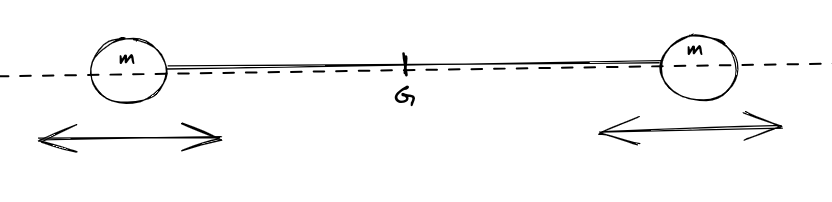
\includegraphics[scale=0.5]{ch9-3_1.png}
        \end{center}
        And here is a sketch of the Morse potential
        \begin{center}
            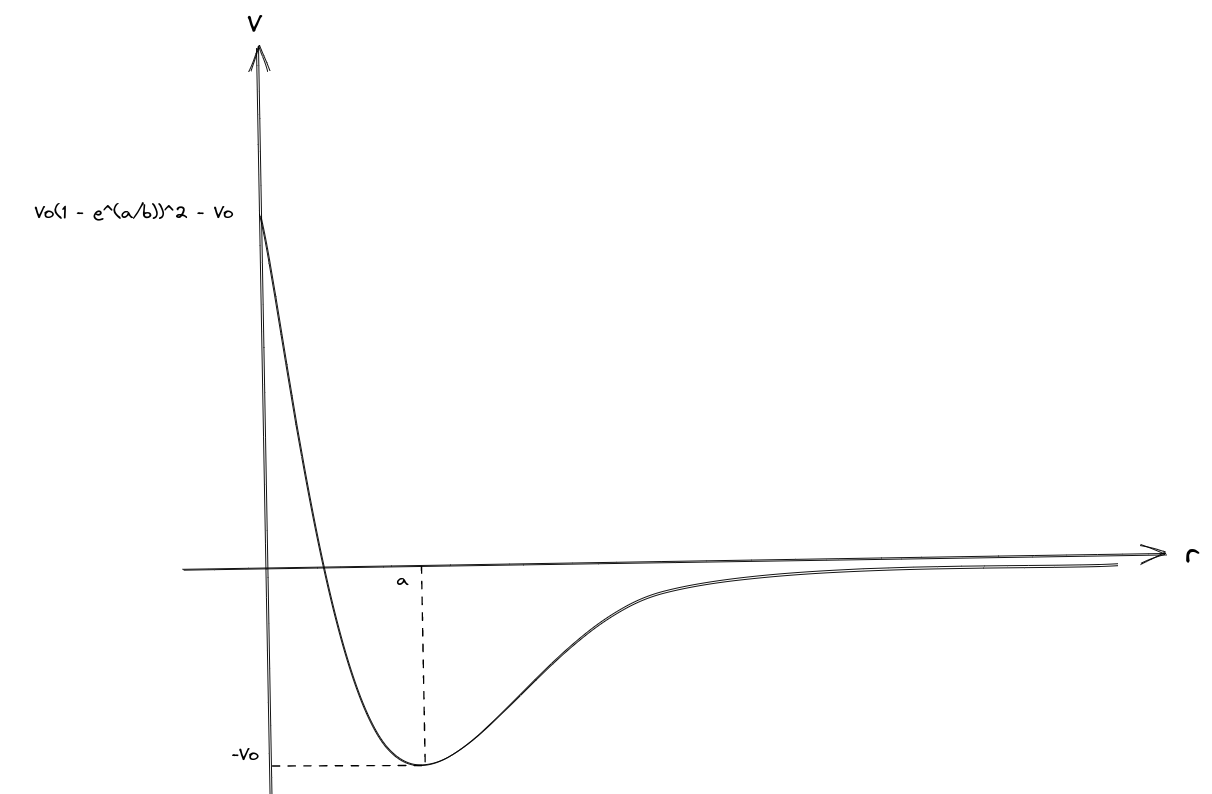
\includegraphics[scale=0.3]{ch9-3_2.png}
        \end{center}

        Now, we want to show that there is a single equilibrium configuration
        and that it's stable. The equilibrium point will happen when $dV/dr=0$
        then we calculate the following
        \begin{align*}
            \frac{dV}{dr} &= \frac{2V_0}{b}(e^\frac{a-r}{b})(1 - e^\frac{a-r}{b})
        \end{align*}
        and we want that
        \begin{align*}
            (e^\frac{a-r}{b})(1 - e^\frac{a-r}{b}) &= 0\\
            e^\frac{a-r}{b} - e^\frac{2(a-r)}{b} &= 0
        \end{align*}
        This equation is satisfied only when $r = a$ so the system has only
        one equilibrium point. Let's now show that this is a stable point by
        showing that $d^2V/dt^2 > 0$ i.e. it's a minimum, we have that
        \begin{align*}
            \frac{d^2V}{dr^2} &= -\frac{2V_0}{b^2}(e^\frac{a-2r}{b})
            (e^\frac{r}{b} - 2e^\frac{a}{b})
        \end{align*}
        so
        \begin{align*}
            \frac{d^2V(a)}{dr^2} &= \frac{2V_0}{b^2}
        \end{align*}
        Therefore we see that ${d^2V(a)}/{dr^2} > 0$ since $V_0$ and $b$ are
        positive constants. From the sketch we did we see this result is
        correct.

        Finally, we want to calculate the angular frequency of the particle.
        Let us calculate a Taylor series approximation to the force applied to
        the particle assuming the Morse potential energy is the only
        contribution then
        \begin{align*}
            F(a) &= -\frac{dV}{dr}(a) \approx 0 - \frac{2V_0}{b^2}(r - a)
        \end{align*}
        Then the approximated equation of motion from Hooke's law is given by
        \begin{align*}
            -k(r-a) &= -\frac{2V_0}{b^2}(r - a)\\
            k &= \frac{2V_0}{b^2}
        \end{align*}
        where $k$ is the spring constant and $r-a$ is the displacement
        because of small oscillation.
        So with this value, we can calculate the angular frequency $\omega$
        as follows
        \begin{align*}
            \omega = \sqrt{\frac{2V_0}{mb^2}}
        \end{align*}
    \end{proof}
	\begin{proof}{\textbf{9.4}}
        Let us suppose that a sphere of radius $r$ was already built, then we
        can equal the densities and calculate the mass of the built sphere
        \begin{align*}
            \frac{m}{4/3\pi r^3} &= \frac{M}{4/3\pi R^3}\\
            m &= M\left(\frac{r}{R}\right)^3
        \end{align*}
        Now suppose we want to add a thin layer of radius $dr$ with mass $dm$
        then in the same way
        \begin{align*}
            \frac{dm}{4 \pi r^2 dr} &= \frac{M}{4/3 \pi R^3}\\
            dm &= \frac{3M r^2}{R^3} dr
        \end{align*}
        To bring this extra mass from infinity to the already-built sphere we
        need to do $Gmdm/r$ work. So to calculate the work of forming the
        entire sphere from nothing we need to replace the values we have for
        $dm$ and $m$ and integrate the expression from $0$ to $R$. The
        self-energy is the negative of the work done.
        \begin{align*}
            V &= -\int_0^R \frac{GM}{r}\frac{r^3}{R^3}\frac{3M r^2}{R^3} dr\\
              &= -\frac{3GM^2}{R^6} \int_0^R r^4 dr\\
              &= -\frac{3GM^2}{R^6}\left[\frac{r^5}{5}\right]_0^R\\
              &= -\frac{3GM^2}{5R}
        \end{align*}
    \end{proof}
	\begin{proof}{\textbf{9.5}}
        The kinetic energy of the system is given by:
        \begin{align*}
            T = \frac{1}{2}Mv^2 + \frac{1}{2}mv^2
        \end{align*}
        where $v$ is the velocity with which the two blocks move along each
        of the inclined planes. 
    
        The gravitational potential energy is given by
        \begin{align*}
            V = mgx\sin\beta - Mgx\sin\alpha = xg(m\sin\beta - M\sin\alpha)
        \end{align*}
        Where $x$ is the displacement of the block and since they
        are connected by a light inextensible string they move the same amount.

        We must now dispose of the constraint forces. Since there is no
        slippage between the string and the two material bodies of the system,
        the total work done by the string on the bodies must be equal
        and opposite to the total work done by the bodies on the string.
        Hence the constraint forces do no work in total.

        Energy conservation, therefore, applies in the form
        \begin{align*}
            \frac{1}{2}(M+m)v^2 + xg(m\sin\beta - M\sin\alpha) = E
        \end{align*}
        Where $E$ is the total energy. If we now differentiate with respect to
        $t$ we get the acceleration of the blocks as follows
        \begin{align*}
            (M+m)v\frac{dv}{dt} + vg(m\sin\beta - M\sin\alpha) = 0\\
            \frac{dv}{dt} = g\left(\frac{M\sin\alpha - m\sin\beta}{M+m}\right)
        \end{align*}

        Finally, to get the tension $T$ in the string we apply Newton's second
        law
        \begin{align*}
            T - mg\sin\beta &= mdv/dt\\
            T &= m(dv/dt + g\sin\beta)\\
            T &= mg\left(\frac{M\sin\alpha - m\sin\beta}{M+m} + \sin\beta\right)\\
            T &= mMg \left(\frac{\sin\alpha + \sin\beta}{M+m}\right)
        \end{align*}
    \end{proof}
\cleardoublepage
	\begin{proof}{\textbf{9.6}}
        From problem 9.1 we know that the potential energy for the system is
        given by
        \begin{align*}
            V &= ga\left(m\sin(\theta) + M\cos(\theta)\right)\\
            V &= mga\left(\sin(\theta) + 2\cos(\theta)\right)
        \end{align*}
        Now we need to determine the kinetic energy $T$ so
        \begin{align*}
            T &= \frac{1}{2}m(a\dot{\theta})^{2} + m(a\dot{\theta})^{2}\\
            T &= \frac{3}{2}m(a\dot\theta)^2
        \end{align*}
        Then the energy conservation equation is given by
        \begin{align*}
            \frac{3}{2}m(a\dot\theta)^2 + 
            mga\left(\sin(\theta) + 2\cos(\theta)\right) = E
        \end{align*}
        And by using the initial conditions where $\theta=\pi/4$ and
        $\dot\theta = 0$ when $t=0$ we can determine that $E = 3mga/\sqrt{2}$.
        Therefore the energy equation in terms of $\theta$ is given by
        \begin{align*}
            \frac{3}{2}a\dot\theta^2 &= \frac{3}{\sqrt{2}}g - g\left(\sin(\theta) + 2\cos(\theta)\right)\\
            \dot\theta^2 &= \frac{g}{3a}\left(3\sqrt{2} - 2\sin(\theta) -
            4\cos(\theta)\right)
        \end{align*}

        Now we want to find the normal reaction of the cylinder on each of the
        particles. By using Newton's second law in the radial direction we can
        determine the cylinder reaction on particle P as follows 
        \begin{align*}
            2mg\cos(\theta) - N_P = 2m\frac{(a\dot\theta)^2}{a}
        \end{align*}
        Then we have that
        \begin{align*}
            N_P &= 2mg\cos(\theta) - 2m\frac{(a\dot\theta)^2}{a}\\
            N_P &= 2mg\cos(\theta) - mg\frac{2}{3}\left(3\sqrt{2} - 2\sin(\theta)
            -4\cos(\theta)\right)\\
            N_P &= \frac{2}{3}mg\left(7\cos(\theta) +  2\sin(\theta) -
                3\sqrt{2}\right)
        \end{align*}
        For the particle $Q$ we have that 
        \begin{align*}
            mg\sin(\theta) - N_Q = m\frac{(a\dot\theta)^2}{a}
        \end{align*}
        And in the same way
        \begin{align*}
            N_Q &= mg\sin(\theta) - m\frac{(a\dot\theta)^2}{a}\\
            N_Q &= mg\sin(\theta) - \frac{mg}{3}\left(3\sqrt{2} - 2\sin(\theta)
            -4\cos(\theta)\right)\\
            N_Q &= \frac{mg}{3}\left(4\cos(\theta) +  5\sin(\theta) -
                3\sqrt{2}\right)
        \end{align*}

        When $N_P = 0$ and $N_Q = 0$ the particles left the cylinder, so by
        solving the equations we get that the particle $Q$ leaves the cylinder
        when $\theta \approx 99^{\circ}$ and particle $P$ leaves the cylinder 
        when $\theta \approx 70^{\circ}$. Here we leave a plot of $N_P$ and
        $N_Q$ against $\theta$ assuming $mg=1$.
        \begin{center}
            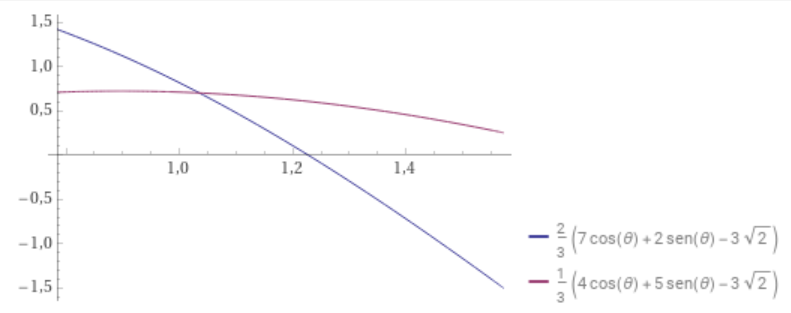
\includegraphics[scale=0.6]{ch9-6.png}
        \end{center}
    \end{proof}
\cleardoublepage
    \begin{proof}{\textbf{9.7}}
        The system we are examining looks like this
        \begin{center}
            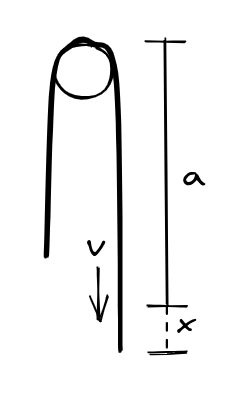
\includegraphics[scale=0.5]{ch9-7.png}
        \end{center}
        Let us first determine the kinetic energy of the rope, since the rope
        is heavy and uniform we can assume that each particle in the rope has
        the same velocity $v = \dot x$ then we have that
        \begin{align*}
            T = \frac{1}{2}M\dot{x}^2
        \end{align*}
        where $M$ is the total mass of the rope.

        The only contribution to the potential energy comes from the uniform
        gravity exerted on the rope so if we suppose the rope is displaced a
        distance $x$ then the mass added to the right side is given by $Mx/2a$
        and also the center of mass is displaced a distance $x$, then
        \begin{align*}
            V = -\bigg(\frac{Mx}{2a}\bigg)gx
        \end{align*}
        We must now show that the constraint forces do no work. The reactions
        exerted by the thin smooth peg on the particles of the rope are always
        perpendicular to the velocities of these particles, these reactions
        therefore do no work. Also, the tension forces exerted by each segment
        of the inextensible string do no work in total. Hence, the constraint
        forces do no work in total.

        Therefore energy conservation can be applied in the form
        \begin{align*}
            \frac{1}{2}M\dot{x}^2 - \frac{Mg}{2a}x^2 = E
        \end{align*}
        and applying the initial conditions $x=0$ and $\dot{x} = 0$ when 
        $t=0$ impliest that $E = 0$ then
        \begin{align*}
            \dot{x} = \sqrt{\frac{g}{a}}x
        \end{align*}

        We want to determine the speed of the rope when it finally leaves the
        peg and this will happen when $x = a$ then
        \begin{align*}
            \dot{x} = \sqrt{ga}
        \end{align*}
    \end{proof}
\cleardoublepage
    \begin{proof}{\textbf{9.8}}
        The system we are examining looks like this
        \begin{center}
            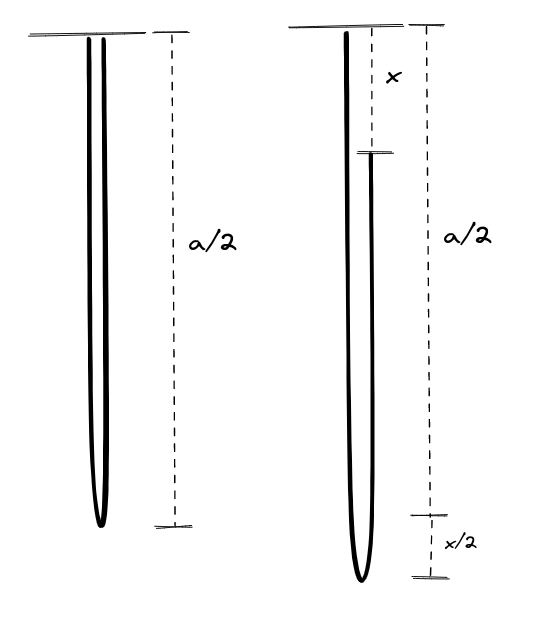
\includegraphics[scale=0.4]{ch9-8.png}
        \end{center}
        Let us first determine the kinetic energy of the rope, the mass of the
        right side of the rope (the one that falls) changes with the distance
        $x$ then the kinetic energy is given by
        \begin{align*}
            T &= \frac{1}{2}\Bigg(\frac{M(a/2 - x/2)}{a}\Bigg)v^2\\
            T &= \frac{1}{4}M\Bigg(1 - \frac{x}{a}\Bigg)v^2
        \end{align*}
        where $M$ is the total mass of the rope.

        The only contribution to the potential energy comes from the uniform
        gravity exerted on the rope so if we suppose the rope is displaced a
        distance $x$ on the right side then
        \begin{align*}
            V &= -\bigg(\frac{M(a/2 + x/2)}{a}\bigg)g\bigg(\frac{a/2 + x/2}{2}\bigg)
            - \bigg(\frac{M(a/2 - x/2)}{a}\bigg)g\bigg(\frac{a/2 - x/2}{2} + x\bigg)\\
            V &= -\frac{Mg}{a}\bigg[\bigg(\frac{a}{2} + \frac{x}{2}\bigg)
            \bigg(\frac{a}{4} + \frac{x}{4}\bigg)
            + \bigg(\frac{a}{2} - \frac{x}{2}\bigg)
            \bigg(\frac{a}{4}+\frac{3x}{4}\bigg)\bigg]\\
            V &= -\frac{Mg}{4a}\bigg(a^2 + 2ax - x^2\bigg)
        \end{align*}
        Assuming the constraint forces do not work the energy conservation can
        be applied in the form
        \begin{align*}
            \frac{1}{4}M\Bigg(1 - \frac{x}{a}\Bigg)v^2
            -\frac{Mg}{4a}\bigg(a^2 + 2ax - x^2\bigg) = E
        \end{align*}
        and applying the initial conditions $x=0$ and $v = 0$ when 
        $t=0$ implies that $E = -Mga/4$ then we have that the velocity of the
        free end when it has descended by a distance $x$ is
        \begin{align*}
            \frac{1}{4}M\Bigg(1 - \frac{x}{a}\Bigg)v^2
            -\frac{Mg}{4a}\bigg(a^2 + 2ax - x^2\bigg) &= -\frac{Mga}{4}\\
            \Bigg(1 - \frac{x}{a}\Bigg)v^2
            -\frac{g}{a}\bigg(a^2 + 2ax - x^2\bigg) &= -ga\\
            \Bigg(1 - \frac{x}{a}\Bigg)v^2 &= 
            -ga +\frac{g}{a}\bigg(a^2 + 2ax - x^2\bigg)\\
            v^2 &=  \frac{gx(2a - x)}{a-x} 
        \end{align*}
        On differentiating again we get the acceleration as follows
        \begin{align*}
            \frac{dv}{dt} = \frac{g(2a^2-2ax+x^2)}{2(a-x)^2}
        \end{align*}
        If we subtract $g$ from both sides we get that
        \begin{align*}
            \frac{dv}{dt}-g &= g\bigg(\frac{(2a^2-2ax+x^2)}{2(a-x)^2} - 1\bigg)\\
            \frac{dv}{dt}-g &= g\bigg(\frac{x(2a-x)}{2(a-x)^2}\bigg)
        \end{align*}
        Where $\frac{x(2a-x)}{2(a-x)^2} > 0$ for $0 < x < a$ then the
        acceleration always exceeds $g$. Finally, if $dv/dt = 5g$ we get that
        \begin{align*}
            5g &= \frac{g(2a^2-2ax+x^2)}{2(a-x)^2}\\
            0 &= 8a^2 - 18ax + 9x^2\\
            x &= \frac{2a}{3} \quad\text{ and }\quad x = \frac{4a}{3}
        \end{align*}
        But given that $x$ cannot exceed $a$ it must happen that $x = 2a/3$.
        So the free end has fallen $2a/3$ when the acceleration is $5g$.
    \end{proof}
\cleardoublepage
    \begin{proof}{\textbf{9.9}}
        The system we are examining looks like this
        \begin{center}
            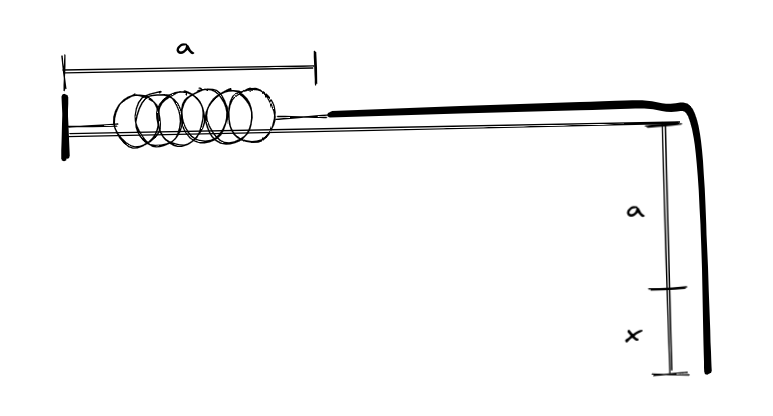
\includegraphics[scale=0.5]{ch9-9.png}
        \end{center}
        Let us first determine the kinetic energy of the rope, since the rope
        is heavy and uniform we can assume that each particle in the rope has
        the same velocity $v = \dot x$ then we have that
        \begin{align*}
            T = \frac{1}{2}M\dot{x}^2
        \end{align*}
        where $M$ is the mass of the rope.

        The contributions to the potential energy come from the uniform
        gravity exerted on the free end of the rope and from the potential
        energy stored in the spring then
        \begin{align*}
            V &= -\bigg(\frac{Mx}{4a}\bigg)g\bigg(a + \frac{x}{2}\bigg)
            + \frac{1}{2}\bigg(\frac{Mg}{2a}\bigg)x^2\\
            V &= \bigg(\frac{Mg}{4a}\bigg)\bigg(-xa - \frac{x^2}{2} + x^2\bigg)\\
            V &= \bigg(\frac{Mg}{8a}\bigg)x(x -2a)
        \end{align*}
        where $\frac{Mg}{2a}$ is the spring constant and we are supposing a
        small displacement $x$ as shown above, which implies a negative
        gravitational potential energy and positive potential energy stored
        in the spring.

        Assuming the table is smooth and the spring is light then the
        constraint forces do not work and so the energy conservation can be
        applied in the form
        \begin{align*}
            \frac{1}{2}M\dot{x}^2 +
            \bigg(\frac{Mg}{8a}\bigg)x(x -2a) = E
        \end{align*}
        Applying the initial conditions $x=0$ and $\dot{x} = 0$ when 
        $t=0$ implies that $E = 0$ then we have that the velocity of the
        free end when it has descended by a distance $x$ is
        \begin{align*}
            \frac{1}{2}M\dot{x}^2 +
            \bigg(\frac{Mg}{8a}\bigg)x(x -2a)
            &= 0\\
            \dot{x}^2 +
            \bigg(\frac{g}{4a}\bigg)x(x -2a)
            &= 0\\
            \dot{x}^2 &=
            \bigg(\frac{g}{4a}\bigg)x(2a - x)
        \end{align*}
        By differentiating this expression we can get the motion equation as
        follows
        \begin{align*}
            2\frac{dx}{dt}\frac{d^2x}{dt^2} &=
            \bigg(\frac{g}{4a}\bigg)(2a - 2x)\frac{dx}{dt}\\
            \frac{d^2x}{dt^2} &= \bigg(\frac{g}{4a}\bigg)(a - x)\\
            \frac{d^2(x-a)}{dt^2} + \bigg(\frac{g}{4a}\bigg)(x-a) &= 0\\
        \end{align*}
        The equation is the one of a simple harmonic motion around the initial
        point $a$ as we wanted. 
        Assuming $\Omega^2 = g/4a$ the period is given by
        \begin{align*}
            \tau = 4\pi\sqrt{\frac{a}{g}}
        \end{align*}
        Finally, the solution to the above equation is of the form
        \begin{align*}
            x - a = A\cos\Omega t + B \sin \Omega t
        \end{align*}
        From the initial conditions $x = 0$ when $t=0$ we have that $A = -a$
        and from the initial condition $\dot{x} = 0$ when $t=0$ we have that
        $B = 0$ then the final equation is given by
        \begin{align*}
            x - a = -a\cos\Omega t
        \end{align*}
        Therefore the amplitude of the motion is $a$.
    \end{proof}
\cleardoublepage
    \begin{proof}{\textbf{9.10}}
        We want to compute first the energy equation before the circular hoop
        loses $h$ altitude then the kinetic energy is given by
        \begin{align*}
            T_i &= \frac{1}{2}Mv_i^2 + \frac{1}{2}I\omega_i^2\\
            T_i &= \frac{1}{2}Mv_i^2 + \frac{1}{2}Mb^2\bigg(\frac{v_i}{b}\bigg)^2\\
            T_i &= Mv_i^2
        \end{align*}
        Where $M$ is the mass of the hoop, $I = Mb^2$ is the moment of inertia
        (from the appendix) and $\omega_i = v_i/b$ is the initial angular
        velocity ($b$ is the hoop's radius).

        The contribution to the potential energy come from the uniform gravity
        exerted to the hoop then.
        \begin{align*}
            V_i = Mgh
        \end{align*}

        Assuming the hoop is rolling without slipping the velocity of the
        bottom point i.e the one in contact with the surface is 0 and in
        consequence there is no displacement so the work done by the constraint
        force is 0 and therefore energy conservation for the initial
        state can be applied in the form
        \begin{align*}
            Mv_i^2 + Mgh = E_i
        \end{align*}

        On the other hand, we can compute the energy conservation equation for
        the final state as follows
        \begin{align*}
            Mv_f^2 = E_f
        \end{align*}
        Where in this case the kinetic energy is computed with the final
        velocity $v_f$ and since we took as a reference point the final state,
        the potential energy is 0 in this case.
        Finally, since we assume the energy is conserved we have that $E_i$
        must be equal to $E_f$ then the final velocity is given by
        \begin{align*}
            Mv_i^2 + Mgh &= Mv_f^2\\
            v_f^2 &= v_i^2 + gh
        \end{align*}  
    \end{proof}
\cleardoublepage
    \begin{proof}{\textbf{9.11}}
        Suppose that, at time $t$, the ball has displacement $x$ down the
        plane (from some reference configuration) and that the center of mass 
        $G$ of the ball has velocity $v$ down the plane. The angular velocity
        $\omega$ of the ball is then determined by $\omega = v/b$ where $b$
        is the radius of the ball. The kinetic energy of the ball is
        therefore
        \begin{align*}
            T &= \frac{1}{2}Mv^2 + \frac{1}{2}I\omega^2\\
            T &= \frac{1}{2}Mv^2
            + \frac{1}{2}\bigg(\frac{2}{5}Mb^2\bigg)\bigg(\frac{v}{b}\bigg)^2\\
            T &= \frac{7}{10}Mv^2 
        \end{align*}
        Where we assumed the ball is a sphere with $I = \frac{2}{5}Mb^2$.

        The contributions to the potential energy come from the uniform
        gravity exerted on the ball then
        \begin{align*}
            V = -Mgx\sin(\alpha)
        \end{align*}
        We must now dispose of the constraint forces. The reaction forces that
        the inclined plane exerts on the ball act on particles of the ball
        which, because of the rolling condition, have zero velocity.
        These reaction forces, therefore, do no work. Also, the internal forces
        that keep the ball rigid do no work in total. Hence the constraint
        forces do no work in total.
        
        So the energy conservation equation is given by
        \begin{align*}
            \frac{7}{10}Mv^2 - Mgx\sin(\alpha) = E 
        \end{align*}
        Finally, if we differentiate the energy conservation equation we get
        the acceleration as we wanted
        \begin{align*}
            \frac{7}{5}Mv\frac{dv}{dt} - Mgv\sin(\alpha) &= 0\\
            \frac{dv}{dt} &= \frac{5g\sin(\alpha)}{7}
        \end{align*}
    \end{proof}
\cleardoublepage
    \begin{proof}{\textbf{9.12}}
        The system we are examining looks like this
        \begin{center}
            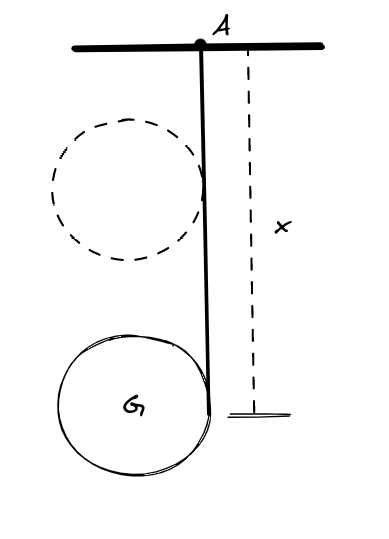
\includegraphics[scale=0.4]{ch9-12.png}
        \end{center}
        The string does no work on the yo-yo because the yo-yo descends without
        slipping so the yo-yo particles in contact with the string have 0
        velocity so they have 0 displacement and hence they do no work.

        Suppose that, at time $t$, the cylinder has displacement $x$ down the
        fixed point $A$ and that the center of mass $G$ of the cylinder has velocity
        $v$. Then the angular velocity $\omega$ of the cylinder is then
        determined by $\omega = v/a$ where $a$ is the radius of the cylinder.
        The kinetic energy of the cylinder is therefore
        \begin{align*}
            T &= \frac{1}{2}Mv^2 +
            \frac{1}{2}\bigg(\frac{1}{2}Ma^2\bigg)\omega^2\\
            T &= \frac{1}{2}Mv^2 +
            \frac{1}{4}Ma^2\bigg(\frac{v}{a}\bigg)^2\\
            T &= \frac{3}{4}Mv^2
        \end{align*}
        Where we assumed the yo-yo is a circular disk with a moment of inertia
        of $I = \frac{1}{2}Ma^2$.

        The contribution to the potential energy come from the uniform
        gravity exerted on the yo-yo then
        \begin{align*}
            V = -Mgx
        \end{align*}

        As we said, the reaction forces of the string because of the rolling
        condition do not work.
        Also, the internal forces that keep the cylinder rigid do no work in
        total.
        Hence the constraint forces do no work in total.

        So the energy conservation equation is given by
        \begin{align*}
            \frac{3}{4}Mv^2 - Mgx = E 
        \end{align*}
        Finally, if we differentiate the energy conservation equation we get
        the acceleration as we wanted
        \begin{align*}
            \frac{3}{2}Mv\frac{dv}{dt} - Mgv &= 0\\
            \frac{dv}{dt} &= \frac{2}{3}g
        \end{align*}

    \end{proof}
    \begin{proof}{\textbf{9.13}}
        Let us first compute the kinetic energy at the initial state of the
        system where the radius is $a$ (we are assuming the roll of paper is
        rolling without slipping) then
        \begin{align*}
            T_a &= \frac{1}{2}MV^2
            + \frac{1}{2}\bigg(\frac{1}{2}Ma^2\bigg)\bigg( \frac{V}{a} \bigg)^2\\
            T_a &= \frac{3}{4}MV^2
        \end{align*}
        Where we used that $M$ is the initial mass of the roll,
        the moment of inertia is $I = \frac{1}{2}Ma^2$ and the angular velocity
        of the roll is $\omega = V/a$.

        Also, we determine the gravitational potential energy for the initial
        state of the system as
        \begin{align*}
            V_a = Mga
        \end{align*}

        Now we are interested in determining what happens when the roll has 
        increased its radius to $b$ then the kinetic energy is given by
        \begin{align*}
            T_b &= \frac{1}{2}\bigg(M\frac{b^2}{a^2}\bigg)v^2
            + \frac{1}{2}\bigg(\frac{1}{2}\bigg(M\frac{b^2}{a^2}\bigg)b^2\bigg)
            \bigg( \frac{v}{b} \bigg)^2\\
            T_b &= \frac{3}{4}\bigg(M\frac{b^2}{a^2}\bigg)v^2
        \end{align*}
        And the potential energy of the system is
        \begin{align*}
            V_b = M\frac{b^3}{a^2}g
        \end{align*}
        Where we used that the mass of the roll when the radius has increased
        to $b$ is $Mb^2/a^2$.
 
        Given that the roll is rolling without slipping the particles in
        contact with the horizontal floor have zero velocity and therefore
        zero displacements, this is saying that the reaction forces do not work.
        Also, the internal forces of the roll do not work and hence
        the constraint forces do not work in total.

        So the energy conservation equation can be applied and it must be
        conserved between the two states we are considering hence from
        the equation we can compute the final velocity as follows
        \begin{align*}
            \frac{3}{4}MV^2 + Mga
            &= \frac{3}{4}\bigg(M\frac{b^2}{a^2}\bigg)v^2 + M\frac{b^3}{a^2}g\\
            \bigg(\frac{b^2}{a^2}\bigg)v^2
            &= V^2 + \frac{4}{3}ga - \frac{4}{3}\frac{b^3}{a^2}g\\
            v^2 &= \frac{a^2}{b^2}V^2
            + \frac{4}{3}\frac{a^3}{b^2}g - \frac{4}{3}bg\\
            v^2 &= \frac{a^2}{b^2}V^2
            + g\frac{4}{3}\bigg(\frac{a^3}{b^2} - b\bigg)\\
        \end{align*}

        Finally, when the roll comes to rest the radius is given by
        \begin{align*}
            0 &= \frac{a^2}{b^2}V^2
            + g\frac{4}{3}\bigg(\frac{a^3}{b^2} - b\bigg)\\
            \frac{b^3 - a^3}{b^2} &= \frac{1}{g}\frac{3}{4}\frac{a^2}{b^2}V^2\\
            b^3 &= \frac{a^2}{g}\frac{3}{4}V^2 + a^3\\
            b &= a\bigg(\frac{3}{4}\frac{V^2}{ag} + 1\bigg)^{1/3}\\
        \end{align*}        
    \end{proof}
\cleardoublepage
    \begin{proof}{\textbf{9.14}}
        The system we are examining looks like this
        \begin{center}
            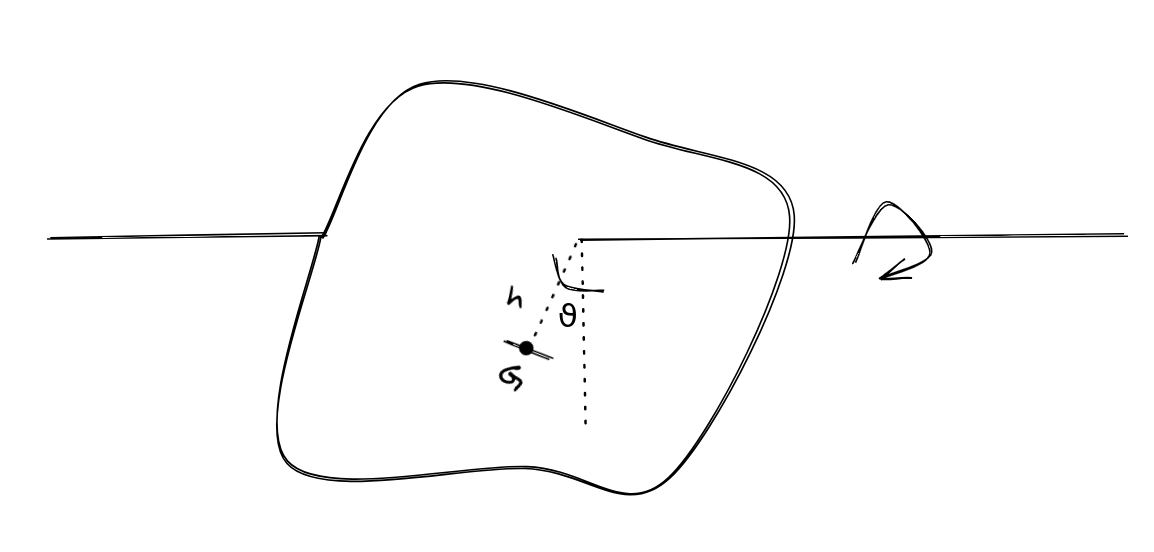
\includegraphics[scale=0.35]{ch9-14.png}
        \end{center}
        where $G$ is the center of mass of the body and theta is the angular
        displacement from the vertical line.

        In this configuration, the kinetic energy looks like 
        \begin{align*}
            T = \frac{1}{2}I\dot{\theta}^2
        \end{align*}
        where $\dot{\theta}$ is the angular velocity and $I$ is the moment
        of inertia of the body.
        Also, the gravitational potential energy is given by
        \begin{align*}
            V = - mgh\cos\theta
        \end{align*}
        Given that the body rotates freely, there are no constraint forces
        and therefore the energy conservation equation is given by
        \begin{align*}
            \frac{1}{2}I\dot{\theta}^2 - mgh\cos\theta = E
        \end{align*}
        By differentiating this equation we get that
        \begin{align*}
            I\dot{\theta}\ddot{\theta} + mgh\dot{\theta}\sin\theta &= 0\\
            I\ddot{\theta} + mgh\sin\theta &= 0
        \end{align*}
        Since we are assuming a set of small oscillations we can replace
        $\sin\theta \approx \theta$ and then the equation becomes
        \begin{align*}
            \ddot{\theta} + \frac{mgh}{I}\theta &= 0
        \end{align*}
        Finally, we know that the oscillation's period in this case is given by
        \begin{align*}
            \tau &= 2\pi\bigg(\frac{I}{mgh}\bigg)^{1/2}
        \end{align*}        
        where we used that $\Omega^2 = \frac{mgh}{I}$.
         
        Now we want to analyze a system analogous to the previous general case
        where the body is a rod of length $2a$ and the distance from it's
        center of mass (the middle of the rod) to the axis of rotation is $b$.

        First, we need to compute the moment of inertia as follows
        \begin{align*}
            I &= \int_{-a+b}^{a+b} \frac{m}{2a}r^2 dr\\
            &= \frac{m}{2a}\bigg[\frac{2}{3}(a^3 + 3ab^2)\bigg]\\
            &= \frac{m}{3}(a^2 + 3b^2)
        \end{align*}        
        Here, we assumed the density of the rod is $m/2a$.

        Finally, we can replace the values in the previous equation and compute
        the period of small oscillations for the rod case as follows.
        \begin{align*}
            \tau &= 2\pi\bigg(\frac{a^2+3b^2}{3gb}\bigg)^{1/2}
        \end{align*}        
 
    \end{proof}

\end{document}






















